%% Figura cuerpo B1: inflación interanual en el Reino Unido y Estados Unidos (generada por Code/datos_3A5.py)
\documentclass[tikz,border=3pt]{standalone}
\usepackage[T1]{fontenc}
\usepackage[utf8]{inputenc}
\usepackage{pgfplots}
\pgfplotsset{compat=1.18}
\begin{document}
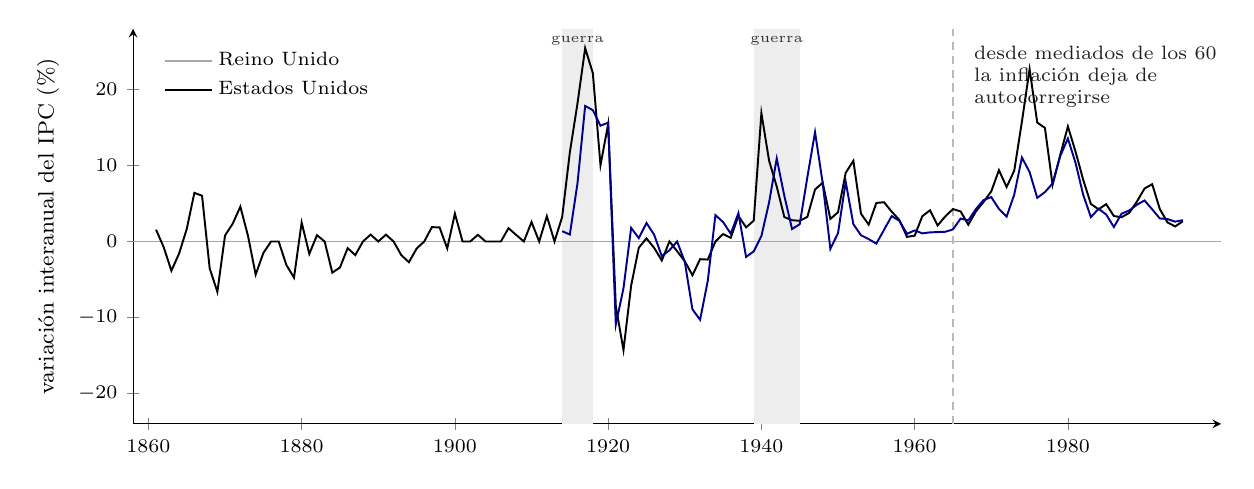
\begin{tikzpicture}[font=\footnotesize]
\begin{axis}[
  width=15.4cm, height=6.6cm,
  axis lines=left,
  xmin=1858, xmax=2000, ymin=-24, ymax=28,
  xtick={1860,1880,1900,1920,1940,1960,1980},
  xticklabel style={/pgf/number format/1000 sep=},
  ytick={-20,-10,0,10,20},
  ylabel={variación interanual del IPC (\%)},
  ylabel style={font=\footnotesize},
  tick label style={font=\scriptsize},
  legend style={at={(0.02,0.97)}, anchor=north west, draw=none, fill=none, font=\scriptsize},
  legend cell align=left,
  clip=false]
\fill[gray!14] (axis cs:1914,-24) rectangle (axis cs:1918,28);
\fill[gray!14] (axis cs:1939,-24) rectangle (axis cs:1945,28);
\node[gray!40!black, font=\tiny, anchor=south] at (axis cs:1916,24.5) {guerra};
\node[gray!40!black, font=\tiny, anchor=south] at (axis cs:1942,24.5) {guerra};
\addplot[gray!70, thin] coordinates {(1858,0) (2000,0)};
\draw[densely dashed, gray!55] (axis cs:1965,-24) -- (axis cs:1965,28);
\node[anchor=north west, align=left, font=\scriptsize, gray!25!black] at (axis cs:1966.5,27)
  {desde mediados de los 60\\la inflación deja de\\autocorregirse};
\addplot[black, line width=0.7pt] coordinates { (1861,1.55) (1862,-0.76) (1863,-3.85) (1864,-1.60) (1865,1.63) (1866,6.40) (1867,6.02) (1868,-3.55) (1869,-6.62) (1870,0.79) (1871,2.34) (1872,4.58) (1873,0.73) (1874,-4.35) (1875,-1.52) (1876,0.00) (1877,0.00) (1878,-3.08) (1879,-4.76) (1880,2.50) (1881,-1.63) (1882,0.83) (1883,0.00) (1884,-4.10) (1885,-3.42) (1886,-0.88) (1887,-1.79) (1888,0.00) (1889,0.91) (1890,0.00) (1891,0.90) (1892,0.00) (1893,-1.79) (1894,-2.73) (1895,-0.93) (1896,0.00) (1897,1.89) (1898,1.85) (1899,-0.91) (1900,3.67) (1901,0.00) (1902,0.00) (1903,0.88) (1904,0.00) (1905,0.00) (1906,0.00) (1907,1.75) (1908,0.86) (1909,0.00) (1910,2.56) (1911,0.00) (1912,3.33) (1913,0.00) (1914,3.23) (1915,11.72) (1916,18.18) (1917,25.44) (1918,22.17) (1919,10.04) (1920,15.44) (1921,-8.51) (1922,-14.29) (1923,-5.81) (1924,-0.82) (1925,0.41) (1926,-0.83) (1927,-2.50) (1928,0.00) (1929,-1.28) (1930,-2.60) (1931,-4.44) (1932,-2.33) (1933,-2.38) (1934,0.00) (1935,0.98) (1936,0.48) (1937,3.37) (1938,1.86) (1939,2.74) (1940,16.89) (1941,10.65) (1942,7.22) (1943,3.21) (1944,2.80) (1945,2.72) (1946,3.24) (1947,6.84) (1948,7.73) (1949,2.97) (1950,3.85) (1951,9.03) (1952,10.62) (1953,3.65) (1954,2.22) (1955,5.07) (1956,5.17) (1957,3.93) (1958,2.84) (1959,0.61) (1960,0.76) (1961,3.33) (1962,4.10) (1963,2.11) (1964,3.31) (1965,4.27) (1966,3.96) (1967,2.21) (1968,3.97) (1969,5.21) (1970,6.60) (1971,9.39) (1972,7.17) (1973,9.33) (1974,15.78) (1975,22.67) (1976,15.65) (1977,14.95) (1978,7.46) (1979,11.39) (1980,15.14) (1981,11.82) (1982,8.11) (1983,4.94) (1984,4.24) (1985,4.91) (1986,3.35) (1987,3.19) (1988,3.76) (1989,5.24) (1990,6.97) (1991,7.54) (1992,4.26) (1993,2.51) (1994,1.98) (1995,2.66) };
\addlegendentry{Reino Unido}
\addplot[blue!55!black, line width=0.7pt] coordinates { (1914,1.35) (1915,0.92) (1916,7.67) (1917,17.84) (1918,17.28) (1919,15.24) (1920,15.63) (1921,-10.94) (1922,-6.16) (1923,1.79) (1924,0.44) (1925,2.43) (1926,0.90) (1927,-1.93) (1928,-1.15) (1929,0.00) (1930,-2.67) (1931,-8.93) (1932,-10.30) (1933,-5.19) (1934,3.48) (1935,2.55) (1936,1.03) (1937,3.73) (1938,-2.03) (1939,-1.30) (1940,0.72) (1941,5.12) (1942,10.92) (1943,5.97) (1944,1.64) (1945,2.27) (1946,8.48) (1947,14.39) (1948,7.69) (1949,-0.97) (1950,1.09) (1951,7.86) (1952,2.28) (1953,0.82) (1954,0.31) (1955,-0.28) (1956,1.53) (1957,3.34) (1958,2.73) (1959,1.01) (1960,1.46) (1961,1.07) (1962,1.20) (1963,1.24) (1964,1.28) (1965,1.59) (1966,3.02) (1967,2.77) (1968,4.27) (1969,5.46) (1970,5.84) (1971,4.29) (1972,3.27) (1973,6.18) (1974,11.05) (1975,9.14) (1976,5.74) (1977,6.50) (1978,7.63) (1979,11.25) (1980,13.55) (1981,10.33) (1982,6.13) (1983,3.21) (1984,4.30) (1985,3.55) (1986,1.90) (1987,3.66) (1988,4.08) (1989,4.83) (1990,5.40) (1991,4.23) (1992,3.03) (1993,2.95) (1994,2.61) (1995,2.81) };
\addlegendentry{Estados Unidos}
\end{axis}
\end{tikzpicture}
\end{document}
